
%%%%%%%%%%%%%%%%%%%%%%%%%%%%% Define Article %%%%%%%%%%%%%%%%%%%%%%%%%%%%%%%%%%
\documentclass[conference]{IEEEtran}
%%%%%%%%%%%%%%%%%%%%%%%%%%%%%%%%%%%%%%%%%%%%%%%%%%%%%%%%%%%%%%%%%%%%%%%%%%%%%%%

%%%%%%%%%%%%%%%%%%%%%%%%%%%%% Using Packages %%%%%%%%%%%%%%%%%%%%%%%%%%%%%%%%%%
\usepackage{geometry}
\usepackage{graphicx}
\usepackage{amssymb}
\usepackage{amsmath}
\usepackage{amsthm}
\usepackage{empheq}
\usepackage{mdframed}
\usepackage{booktabs}
\usepackage{lipsum}
\usepackage{graphicx}
\usepackage{color}
\usepackage{psfrag}
\usepackage{pgfplots}
\usepackage{bm}
\usepackage[spanish]{babel}
\usepackage[utf8]{inputenc} % Codificación UTF,8
\usepackage{amsmath}        % Soporte para ecuaciones matemáticas
\usepackage{graphicx}       % Manejo de imágenes
\usepackage{hyperref}       % Hipervínculos
\usepackage{caption}        % Formato para figuras
\usepackage{multirow}
\usepackage{subcaption}
\usepackage{biblatex}
\usepackage{csquotes}
\usepackage{bookmark}
%%%%%%%%%%%%%%%%%%%%%%%%%%%%%%%%%%%%%%%%%%%%%%%%%%%%%%%%%%%%%%%%%%%%%%%%%%%%%%%

% Other Settings

%%%%%%%%%%%%%%%%%%%%%%%%%% Page Setting %%%%%%%%%%%%%%%%%%%%%%%%%%%%%%%%%%%%%%%
\geometry{a4paper, margin=1in}

%%%%%%%%%%%%%%%%%%%%%%%%%% Define some useful colors %%%%%%%%%%%%%%%%%%%%%%%%%%
\definecolor{ocre}{RGB}{243,102,25}
\definecolor{mygray}{RGB}{243,243,244}
\definecolor{deepGreen}{RGB}{26,111,0}
\definecolor{shallowGreen}{RGB}{235,255,255}
\definecolor{deepBlue}{RGB}{61,124,222}
\definecolor{shallowBlue}{RGB}{235,249,255}
%%%%%%%%%%%%%%%%%%%%%%%%%%%%%%%%%%%%%%%%%%%%%%%%%%%%%%%%%%%%%%%%%%%%%%%%%%%%%%%

%%%%%%%%%%%%%%%%%%%%%%%%%% Define an orangebox command %%%%%%%%%%%%%%%%%%%%%%%%
\newcommand\orangebox[1]{\fcolorbox{ocre}{mygray}{\hspace{1em}#1\hspace{1em}}}
%%%%%%%%%%%%%%%%%%%%%%%%%%%%%%%%%%%%%%%%%%%%%%%%%%%%%%%%%%%%%%%%%%%%%%%%%%%%%%%

%%%%%%%%%%%%%%%%%%%%%%%%%%%% English Environments %%%%%%%%%%%%%%%%%%%%%%%%%%%%%
\newtheoremstyle{mytheoremstyle}{3pt}{3pt}{\normalfont}{0cm}{\rmfamily\bfseries}{}{1em}{{\color{black}\thmname{#1}~\thmnumber{#2}}\thmnote{\,,,\,#3}}
\newtheoremstyle{myproblemstyle}{3pt}{3pt}{\normalfont}{0cm}{\rmfamily\bfseries}{}{1em}{{\color{black}\thmname{#1}~\thmnumber{#2}}\thmnote{\,,,\,#3}}
\theoremstyle{mytheoremstyle}
\newmdtheoremenv[linewidth=1pt,backgroundcolor=shallowGreen,linecolor=deepGreen,leftmargin=0pt,innerleftmargin=20pt,innerrightmargin=20pt,]{theorem}{Theorem}[section]
\theoremstyle{mytheoremstyle}
\newmdtheoremenv[linewidth=1pt,backgroundcolor=shallowBlue,linecolor=deepBlue,leftmargin=0pt,innerleftmargin=20pt,innerrightmargin=20pt,]{definition}{Definition}[section]
\theoremstyle{myproblemstyle}
\newmdtheoremenv[linecolor=black,leftmargin=0pt,innerleftmargin=10pt,innerrightmargin=10pt,]{problem}{Problem}[section]
%%%%%%%%%%%%%%%%%%%%%%%%%%%%%%%%%%%%%%%%%%%%%%%%%%%%%%%%%%%%%%%%%%%%%%%%%%%%%%%

%%%%%%%%%%%%%%%%%%%%%%%%%%%%%%% Plotting Settings %%%%%%%%%%%%%%%%%%%%%%%%%%%%%
\usepgfplotslibrary{colorbrewer}
\pgfplotsset{width=8cm,compat=1.9}
%%%%%%%%%%%%%%%%%%%%%%%%%%%%%%%%%%%%%%%%%%%%%%%%%%%%%%%%%%%%%%%%%%%%%%%%%%%%%%%

%%%%%%%%%%%%%%%%%%%%%%%%%%%%%%% Title & Author %%%%%%%%%%%%%%%%%%%%%%%%%%%%%%%%
\author{\IEEEauthorblockN{Daniel Fernando Aranda Contreras, Diana Fernanda Abril Roa, Nicolás Hernández Buitrago,\\ Rafael Miguel Segura Garzon}
\IEEEauthorblockA{Escuela E3T, Universidad Industrial de Santander\\
Correo electrónico: \{daniel2221648, diana2212074, nicolás2204593, rafael2202194 \}@correo.uis.edu.co}}

%%%%%%%%%%%%%%%%%%%%%%%%%%%%%%%%%%%%%%%%%%%%%%%%%%%%%%%%%%%%%%%%%%%%%%%%%%%%%%%
    \begin{document}
        % Título
        \title{\uppercase{Practica No.4. Transformadores monofásicos: Autotransformador}}
        \maketitle
        % Resumen
        % Palabras clave        
        \begin{IEEEkeywords}
            Autotransformador, Transformador monofásico, Pruebas de vacío, Pruebas de cortocircuito, Relación de transformación, 
            Rendimiento, Regulación, Carga resistiva (R), Carga inductiva (L), Carga capacitiva (C), Modelo equivalente
            , Máxima eficiencia, Tensión primaria, Tensión secundaria, Corriente nominal, Factor de potencia, Conexión eléctrica  
            , Potencia de entrada, Potencia de salida.
        \end{IEEEkeywords}
        \section{Objetivos} 
\begin{itemize}
    \item Realizar las pruebas de vacío y de cortocircuito en un transformador monofásico configurado como autotransformador para analizar su comportamiento eléctrico.
    \item Determinar experimentalmente el rendimiento y la regulación del autotransformador bajo diferentes tipos de carga: resistiva, inductiva y capacitiva.
\end{itemize}

\section{Equiops y materiales}
\begin{itemize}
    \item Transformador monofásico.
    \item Voltímetro CA.
    \item Amperímetro CA.
    \item Vatímetro monofásico CA.
    \item Transformador de corriente (CT).
    \item Cargas: resistivas (R), inductivas (L) y capacitivas (C).
\end{itemize}

\section{Introducción}
\text{Los autotransformadores son dispositivos eléctricos que facilitan la modificación de los niveles de tensión dentro de un rango específico de manera eficiente. A diferencia de los transformadores tradicionales, en los autotransformadores los devanados primario y secundario no están completamente aislados, ya que comparten una parte del mismo arrollamiento. Esto resulta en una reducción del material conductor utilizado y en una mejora de la eficiencia del sistema. En este laboratorio, se realizará un estudio de un transformador monofásico funcionando como autotransformador, a través de pruebas experimentales que permitirán evaluar su rendimiento y regulación en diversas condiciones de carga.}

\section{Conclusión}
\text{A lo largo del laboratorio, se estudió el comportamiento de un transformador monofásico operando como autotransformador, evaluando su rendimiento y regulación bajo diferentes condiciones de carga, las cuales tienen una gran influencia en su rendimiento depediendo el tipo de carga, si es una carga RC conectada en paralelo tiende a aunmentar su tension de salida en comparacion con una carga netamente resistiva, mientras que con una carga inductiva conectada en serie su nivel de tension de salida disminuye, pero si conectamos una carga RLC está tiene un comportamiento de compensacion, si las cargas inductivas (L) y capacitivas (C) tienen valores similares.}
        \section{Anexos de la Práctica 5}


\begin{figure}[ht!] % 'h' indica que la imagen se coloca aquí
    \centering
    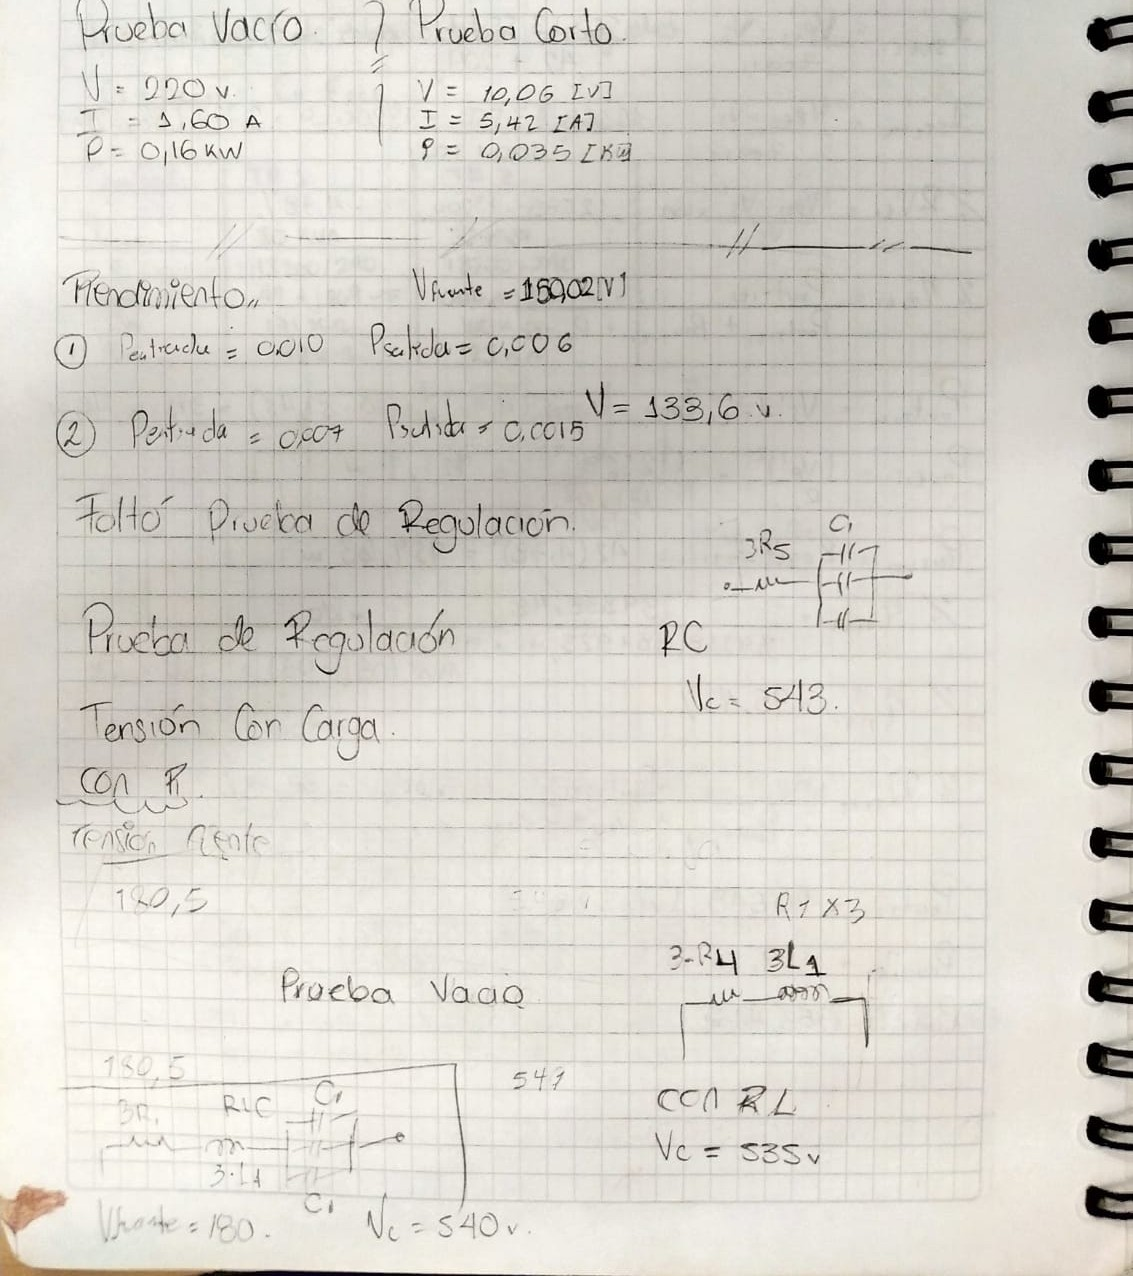
\includegraphics[width=0.48\textwidth]{fot/prac4_hoja de tales.jpg} % Cambia la ruta a tu imagen
    \caption{Hoja de la practica con los resultados de las pruebas.}
    \label{fig:hoja}
\end{figure}


\begin{figure}[ht!] % 'h' indica que la imagen se coloca aquí
    \centering % Centra la imagen
    \begin{subfigure}{0.5\textwidth}
            \centering
            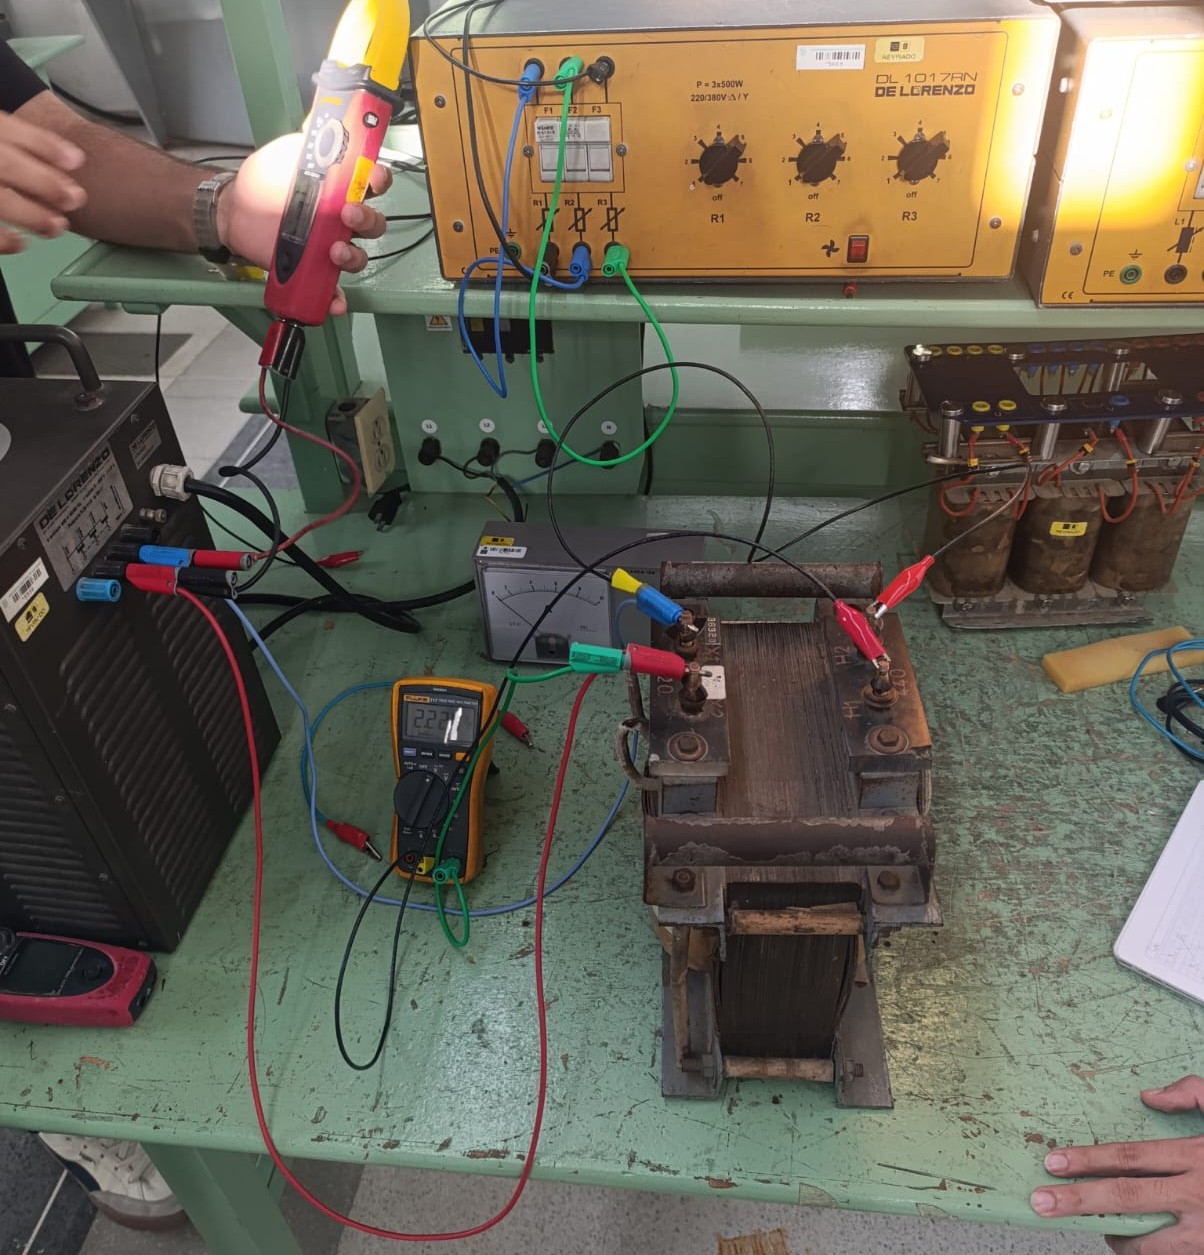
\includegraphics[width=0.8\textwidth]{fot/prac4_autoenvacio.jpeg} % Cambia la ruta a tu imagen
            \caption{Autotransformador en la prueba de vacio (Hay una carga de resistencias en serie que estan desconectadas).}
            \label{fig:prac4_autoenvacio}
    \end{subfigure}
    \hfill % Espacio horizontal entre las subfiguras
    \begin{subfigure}{0.5\textwidth}
        \centering
        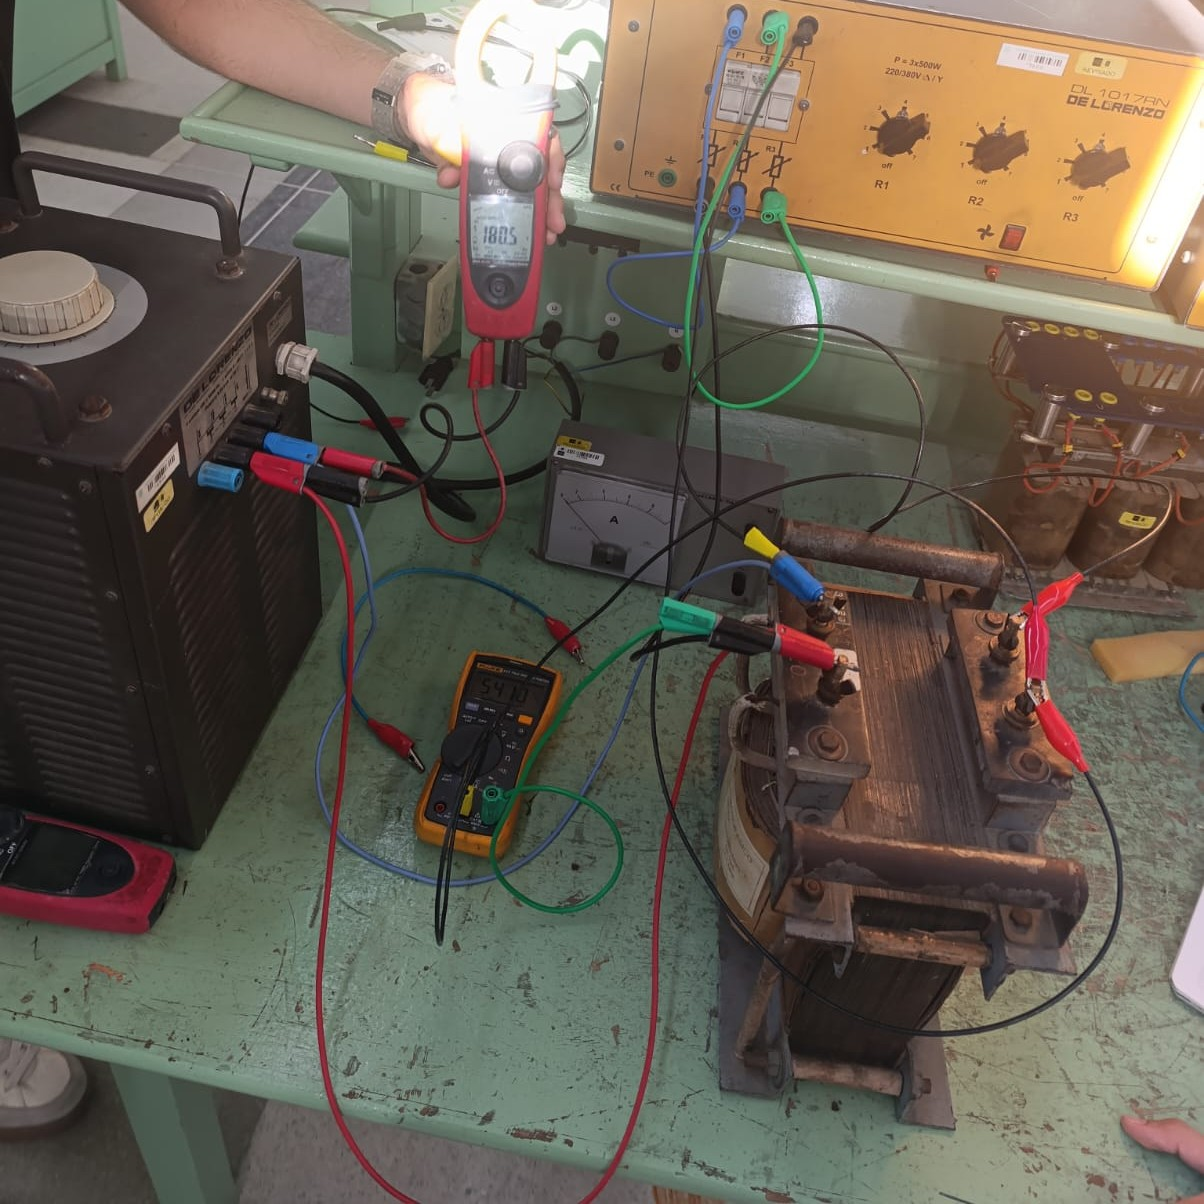
\includegraphics[width=0.8\textwidth]{fot/prac4_autoR_.jpeg} % Cambia la ruta a tu imagen
        \caption{Autotransformador con tres cargas resistivas conectadas en serie.}
        \label{fig:AutoR1}  
    \end{subfigure}
    \label{fig:dos-imagenes}
    \hfill
    \begin{subfigure}{0.5\textwidth} % Corrected missing curly brace
        \centering
        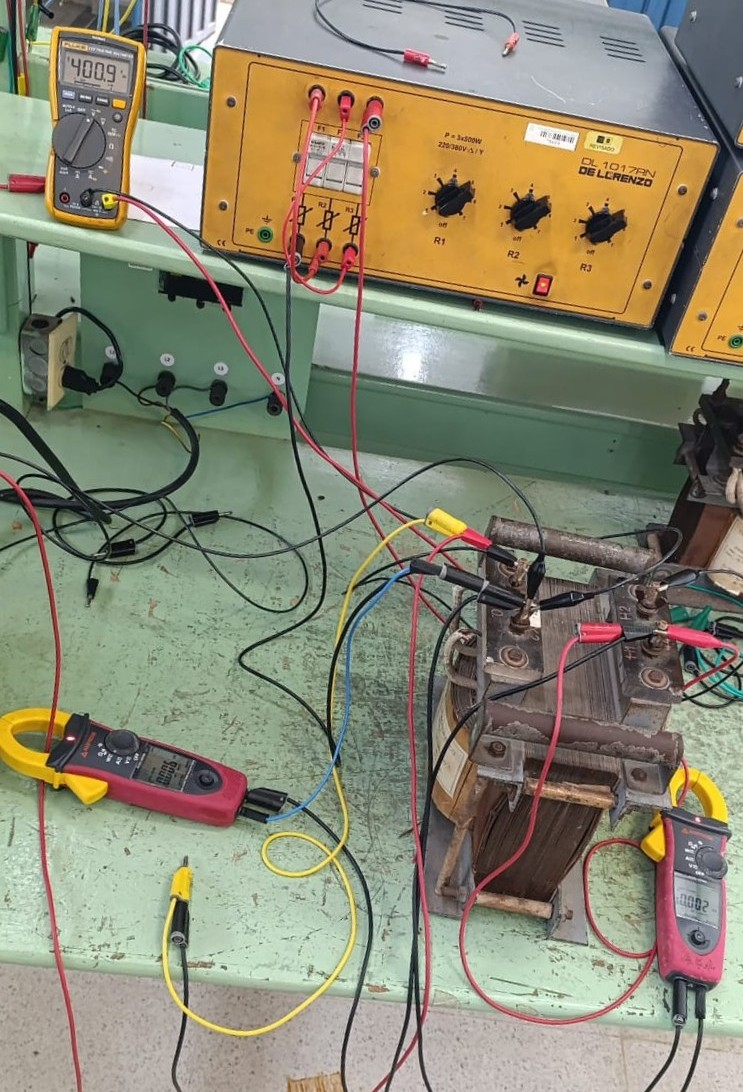
\includegraphics[width=0.8\textwidth]{fot/prac4_rendimiento.jpg} % Cambia la ruta a tu imagen
        \caption{Autotransformador realizando prueba de rendimiento.}
        \label{fig:Autorendimiento}
    \end{subfigure}
\end{figure}
        
        \end{document}  
